
%% 4-5 pages

\section{Results}
In this section the results the study is presented.
The result will be divided into subsections for the result from the survey conducted to establish requirements and the results from the thematic analysis of the interviews conducted to evaluate a prototype of a proposed technical debt management tool.

\subsection{Survey results}
The survey was conducted among proffessionals with various roles in software development projects, with the most common role being "Developer" (90\%) followed by "Tech Lead or Project Manager" (60\%) and "DevOps" (20\%).
The number of respondents was 20 with mixed and somewhat evenly distributed level of experience between "less than 5 years" (40\%), "between 6 and 10 years" (25\%) and "more than 10 years" (35\%).
All but one (95\%) of the respondents were familiar with the term "Technical Debt" indicating that the respondent have a understanding of the concept and thus the required prior knowledge to be able to provive relevant answers in the survey.

In order to understand how technical debt affects the daily work of the respondents and their experience of communicating about and manage technical debt in their current situation, the survey presented nine statements asking the respondents to indicate whether they agree or disagree according to a likert scale. %% TODO: Add ref
The results are presented in figure \ref{fig:statementresult}, where each statement is assigned a letter and the distribution of the answers for each statement represented with a bar in the figure.

\smallskip
\textbf{Statements:}
\begin{enumerate}[label=\alph*)]
  \item I find that technical debt is a problem in my current project.
  \item Technical debt is often necessary in order to deliver in time.
  \item The amount of technical debt in my current project is acceptable.
  \item I have a clear overview of the amount of technical debt in the project.
  \item I have a clear overview of where in the project technical debt is present.
  \item The technical debt in the project is actively managed.
  \item The project team has clear communication about technical debt.
  \item The project team has a clear strategy for how to manage technical debt.
  \item Everyone in the project team are aware of the technical debt strategy.
\end{enumerate}
\smallskip

\begin{figure}[t]
  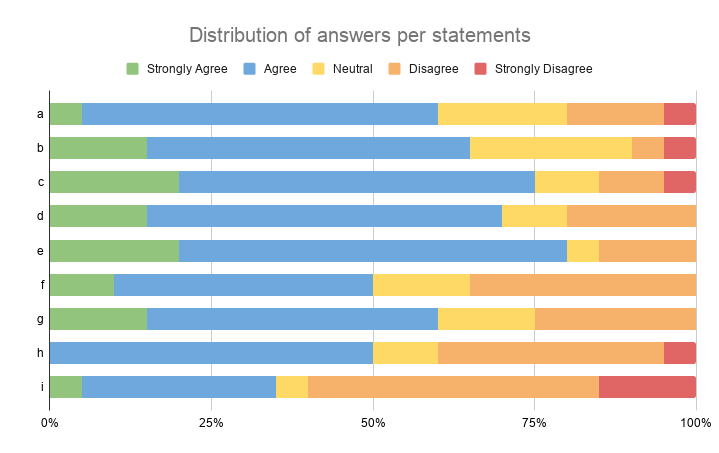
\includegraphics[width=\columnwidth]{StatementAnswers}
  \Description{Chart representing the distribution of answers per statement.}
  \caption[StatementResults]{Chart representing the distribution of answers per statement.}
  \label{fig:statementresult}
  \centering
\end{figure}

The results show that although more than halv of the respondent (60\%) find technical debt to be a problem in their project, a majority (65\%) agree that technical debt is necessary in order to deliver.
Further, most respondents (75\%) consider their current level of debt acceptable.
This indicates that developers are facing the need to balance the problems caused by tecnical debt with the need to deliver in time and that this requires accepting a certain level of technical debt.

A greater part of the respondent indicate that they have a clear overview of both the amount of technical debt (70\%) and where the debt is located in the project (80\%).
However, only half of the respondents work in a project where technical debt is activly managed (50\%) or with a clear strategy for technical debt management (50\%), and a majority (60\%) does not experience that everyone in their team are aware of the technical debt strategy.
This points to a problem with an absence of awareness and communication about thechnical debt in many software development projects.

\subsection{Interviews}
Based on the data collected and analyzed from the survey, a prototype was designed with the goal to be a common source of information about a software development teams strategy and priorities regarding technical debt.